\documentclass[DIN, pagenumber=false, fontsize=11pt, parskip=half]{scrartcl}

\usepackage{amsmath}
\usepackage{amsfonts}
\usepackage{amssymb}
\usepackage{enumitem}
\usepackage[utf8]{inputenc} 
\usepackage[ngerman]{babel} 
\usepackage[T1]{fontenc} 
\usepackage{pgfplots}
\usepackage{xcolor}
\usepackage{listings}
\usepackage{float}
\usepackage{graphicx}
\usepackage{booktabs}
\usepackage{tkz-euclide}
\usepackage{svg}
\usepackage{trfsigns}
\usepackage{mathtools}

\DeclarePairedDelimiter\abs{\lvert}{\rvert}%
\DeclarePairedDelimiter\norm{\lVert}{\rVert}%

\definecolor{mygreen}{RGB}{28,172,0} % color values Red, Green, Blue
\definecolor{mylilas}{RGB}{170,55,241}

\tikzstyle{neuron}=[circle,fill=black!25,minimum size=30pt,inner sep=0pt]

\lstset{language=Matlab,%
    %basicstyle=\color{red},
    breaklines=true,%
    morekeywords={matlab2tikz},
    keywordstyle=\color{blue},%
    morekeywords=[2]{1}, keywordstyle=[2]{\color{black}},
    identifierstyle=\color{black},%
    stringstyle=\color{mylilas},
    commentstyle=\color{mygreen},%
    showstringspaces=false,%without this there will be a symbol in the places where there is a space
    numbers=left,%
    numberstyle={\tiny \color{black}},% size of the numbers
    numbersep=9pt, % this defines how far the numbers are from the text
    emph=[1]{for,end,break},emphstyle=[1]\color{red}, %some words to emphasise
    %emph=[2]{word1,word2}, emphstyle=[2]{style},    
}

\title{Einführung in die Neuroinformatik}
\author{Tim Luchterhand, Paul Nykiel (Gruppe P)}

\begin{document}
    \maketitle
    \section{Autoassoziativer Speicher}
    \lstinputlisting{b12a01.m}
    \begin{figure}[H]
        \centering
        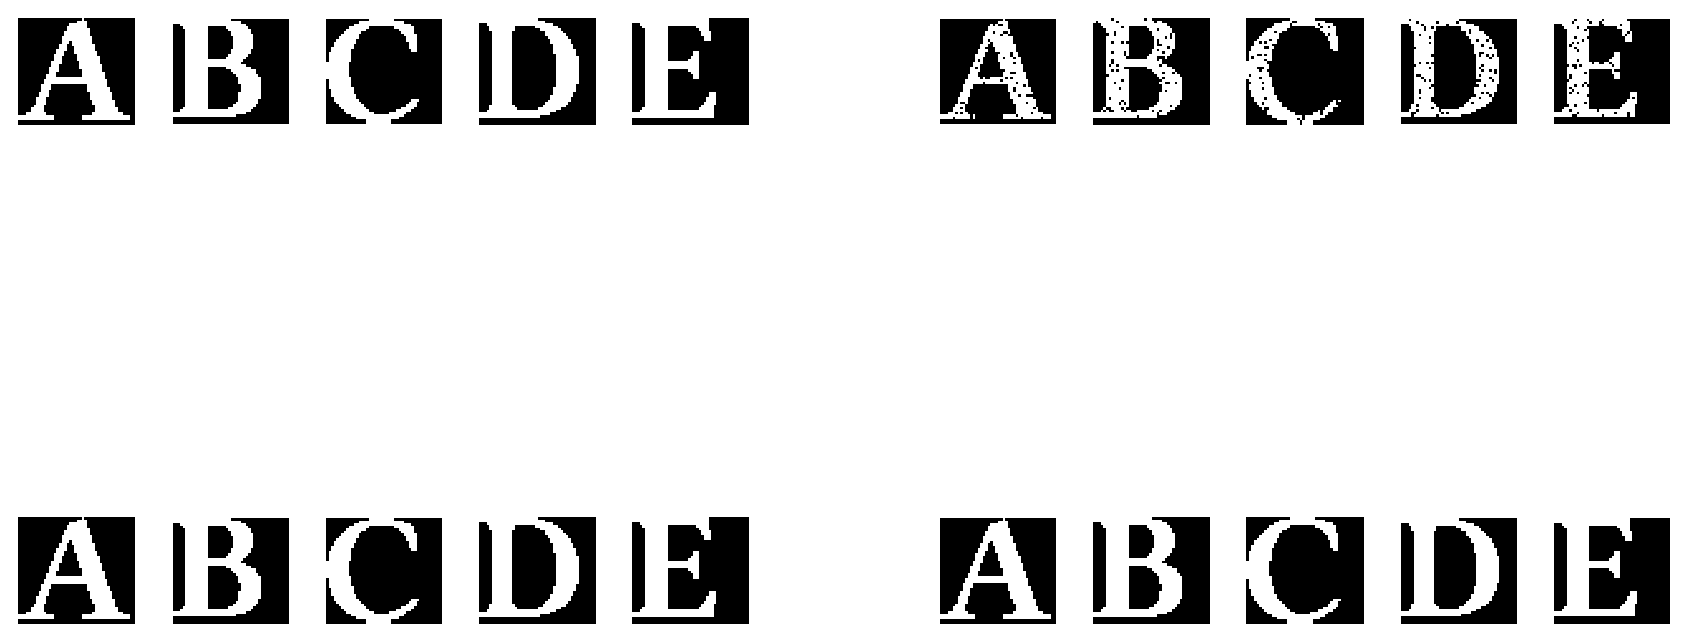
\includegraphics[width=\textwidth]{b12a01.eps}
        \caption{Ausgabe des Matlab-Skripts}
    \end{figure}

    \section{Speicherkapazität}
    \lstinputlisting{b12a02.m}
    \begin{figure}[H]
        \centering
        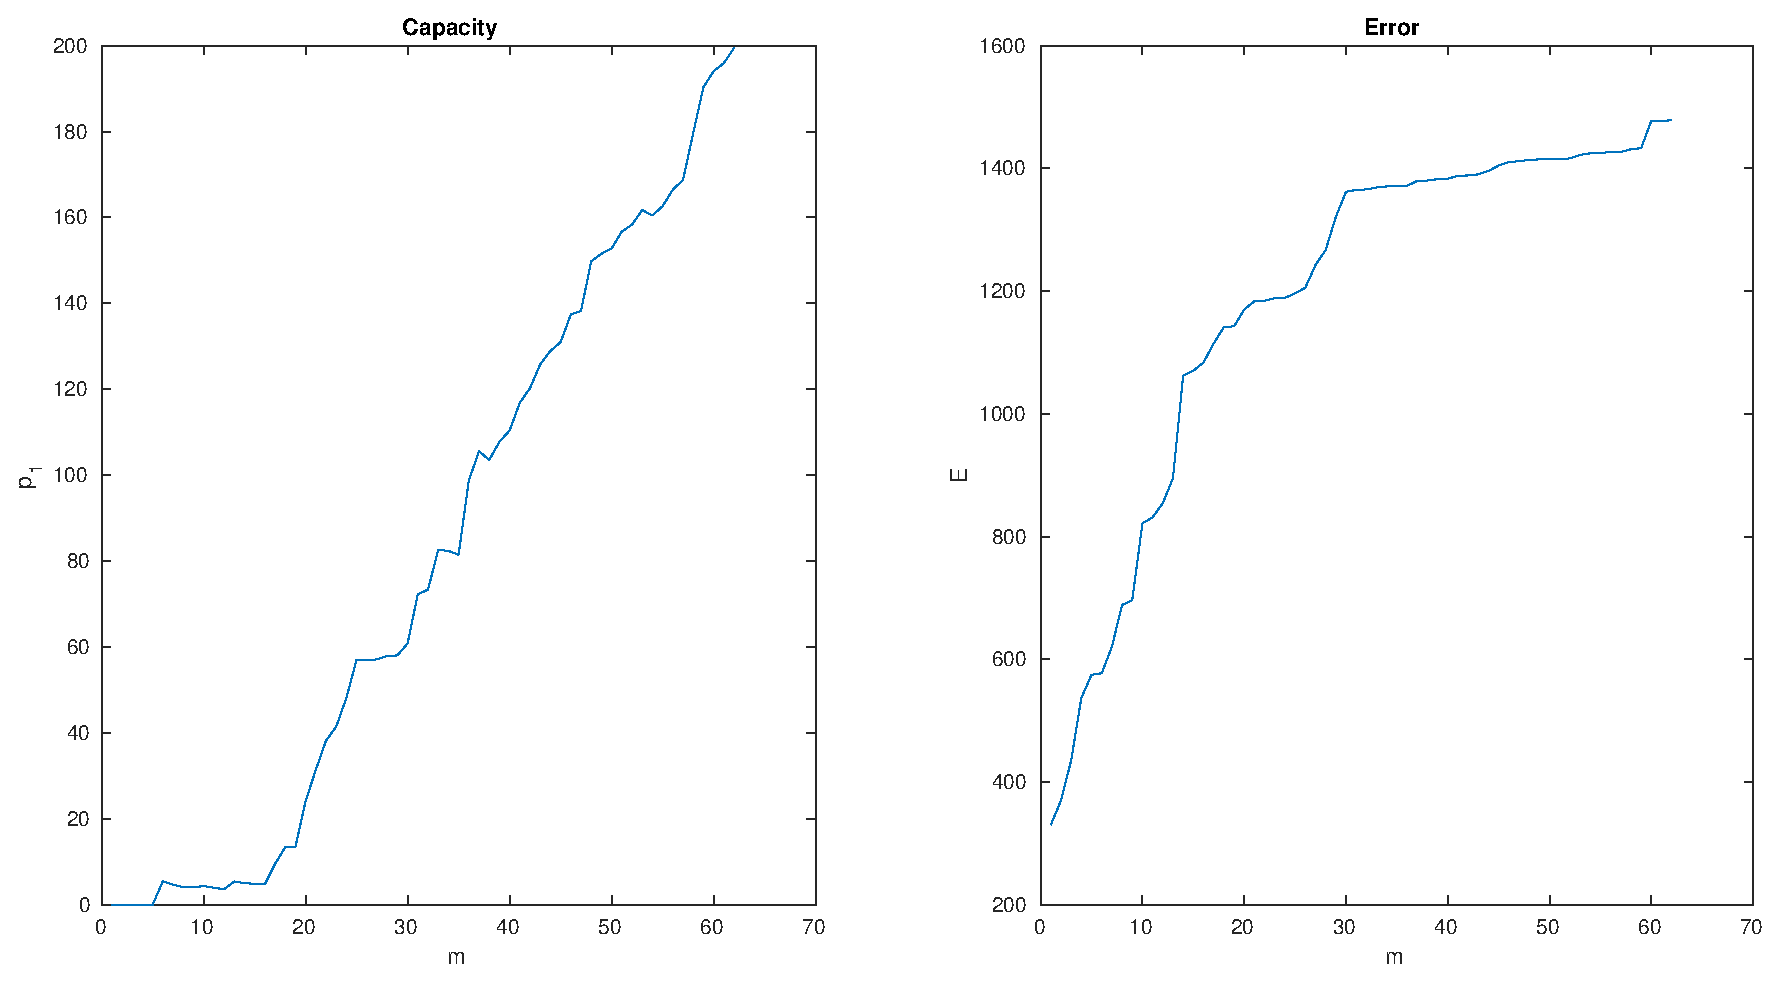
\includegraphics[width=\textwidth]{b12a02.eps}
        \caption{Ausgabe des Matlab-Skripts}
    \end{figure}
\end{document}
